    \documentclass[conference]{IEEEtran}
\IEEEoverridecommandlockouts
% The preceding line is only needed to identify funding in the first footnote. If that is unneeded, please comment it out.
\usepackage{cite}
\usepackage{amsmath,amssymb,amsfonts}
\usepackage{algorithmic}
\usepackage{graphicx}
\usepackage{subfigure}
\usepackage{textcomp}
\usepackage{xcolor}
\usepackage{caption}
\usepackage{geometry}
\usepackage{color}
\usepackage{bm}
\def\BibTeX{{\rm B\kern-.05em{\sc i\kern-.025em b}\kern-.08em
    T\kern-.1667em\lower.7ex\hbox{E}\kern-.125emX}}


\geometry{letterpaper,left=1.91cm,right=1.91cm,top=2.54cm,bottom=1.91cm}
\begin{document}
% ***************************************************************begin********************************************************

\title{Seeing is Sensing - External Observation of \emph{In Vivo} Biological Gradient Field by Tracking Nanoswimmers  }


\author{Kunlun Wu$^{1}$, % <-this % stops a space
	  Yue Sun$^{1}$,
	  Zheng Gong$^{2}$,
	  Xiaorong Ding$^{1}$, and
	  Yifan Chen$^{*1}$

\thanks{$^{1}$K. Wu, X. Ding and Y. Chen are with the School of Life Science and Technology, University of Electronic Science and Technology of China, Chengdu, 611731, China.(*corresponding author e-mail: yifan.chen@uestc.edu.cn).

	  $^{2}$Y. Sun is with the School of Life Science and Technology, University of Electronic Science and Technology of China, Chengdu, 611731, China. He is also with the School of Information Science and Technology, Chengdu University of Technology, Chengdu, 610059, China.

	  $^{3}$Z. Gong is with the School of  Engineering, the University of Waikato, Hamilton, 3240, NewZealand.
      }%

}



\maketitle

\begin{abstract}
This work aims to demonstrate through computational analysis that, by monitoring the trajectory of externally manipulable nanoswimmers (NS), the \emph{in vivo} biological gradient field (BGF) interacting with the NS can be indirectly observed. This observability is fundamental to the recently proposed framework of computational nanobiosensing (CONA) for “smart” cancer detection. We first present a novel NS propagation model to emulate the complex and chaotic NS kinetics inside the capillary network. Next, we propose an efficient control method that is able to employ the NS as in vivo sensors for the measurement of a specific BGF such as blood viscosity. The proposed method, based on the Linear Quadratic Regulator (LQR), effectively stabilizes the signal-to-noise ratio (SNR) induced by the Brownian motion of NS at a level above 10 dB to enhance the accuracy of viscosity estimation.
\end{abstract}

\begin{IEEEkeywords}
\emph{In vivo} sensor, Nanoswimmers, Blood viscosity estimation, Linear Quadratic Regulator.
\end{IEEEkeywords}



\section{Introduction}
Nanoparticle-mediated drug delivery shows great promise in cancer diagnosis \cite{tran2017cancer}. However, without any external guidance, systemic circulation can only bring 0.7{\%} of the injected nanoparticles to the tumor targets \cite{wilhelm2016analysis}. This low efficiency is a key hurdle for translating nanomedicines from the lab into the clinic. From a computational perspective, this sensing process is simply a “brute-force search”, because the nanoparticles (computing agents) can only “detect” a tumor by enumerating all possible pathways in the complex vascular network \cite{shi2019microrobots}. By replacing nanoparticles with externally manipulable nanoswimmers (NS), we have proposed a novel computational nanobiosensing (CONA) framework for “smart” searching of tumors \cite{shi2019perspective}. The presence of a tumor induces changes in some biological gradient fields (BGFs) such as pathological vascular structure, blood velocity and viscosity, pH, enzymatic activity, and homeostatic regulation\cite{shi2019microrobots}, which will subsequently alter the externally measurable properties of NS such as trajectories and aggregation patterns. Computationally, the BGF could be utilized as the “objective function”; the targeted tumor site corresponds to the 
“global optimum”; and the NS are “computing agents”. Thus, NS could cooperate to find the targeted site under the guidance of an external steering field programmed according to specific \emph{in vivo} function optimization algorithms. However, The CONA framework is still hypothetical because BGFs were assumed to be perfectly inferred by measuring the characteristics of NS. The current work aims at exploring the observability of BGF, which is a fundamental problem to be investigated in CONA.

Recent studies have suggested that blood viscosity is a useful BGF parameter for early diagnosis of tumors and other diseases \cite{salve2019design}. Furthermore, with the continuous development of nanotechnology, magnetic nanoparticles have been extensively used as NS because of their great promise in both controllability and flexibility. The motion of NS in the stagnant fluidic environment has already been reported in some works. The influence on the swimming speed of bacterial NS in high-viscosity fluids was modelled in \cite{magariyama2002mathematical}. The swimming characteristics of ferromagnetic microsphere chains in fluidic environments with respect to viscosity were described in \cite{belharet2014study}. However, to the best of our knowledge, there are rarely NS-based sensing methods related to the hemodynamic changes, especially in terms of blood viscosity. The exsiting nanorobotic control strategies are only focused on the controllability but are short of researching the BGF observability.

In this work, we propose a  novel model to emulate the complex and chaotic kinematics of magnetic-nanoparticles-assembled NS in human vessels. Through analysing the average trajectory of several NS released one by one in the time domain, it is able to solve the inverse problem about hemodynamics so as to obtain the estimation of the relative blood viscosity. To further improve the sensing performance, we present a controller that uses the Linear Quadratic Regulator (LQR) for reducing the noise in the viscosity measurement.

The remaining part of this paper is organized as follows: 
In section II, the system models and the motion-based viscosity sensing strategy are presented. Section III introduces the concept of location-dependent signal-to-noise ratio (SNR) and propose the LQR control method to improve the sensing performance. Numerical results are presented in Section IV to verify the effectiveness of the proposed method. Finally, some concluding remarks are drawn in section V.

\newgeometry{letterpaper,left=1.91cm,right=1.91cm,top=1.91cm,bottom=1.91cm}

\begin{figure}
\centering
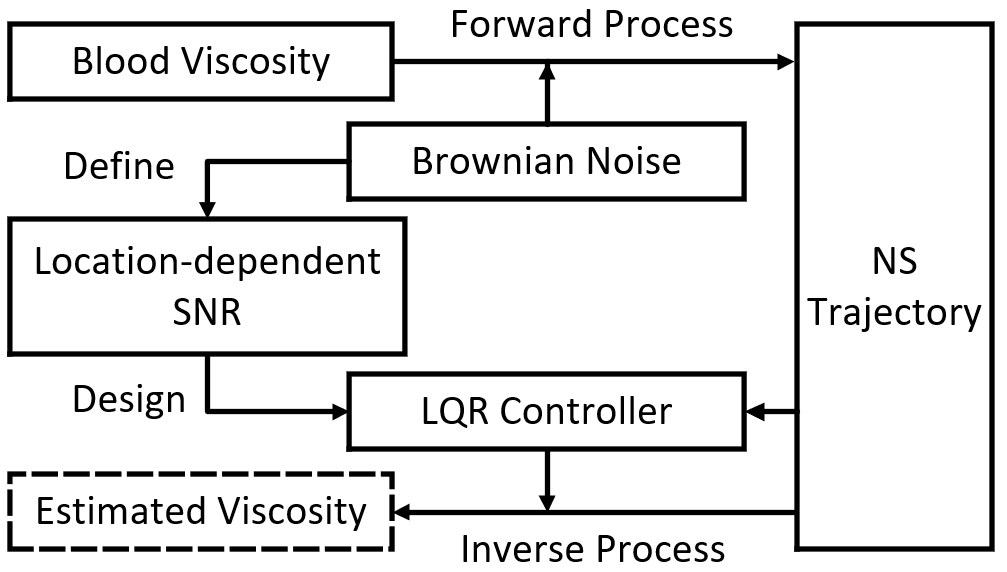
\includegraphics[width=8cm]{fig1.png}
\caption{Framework of the viscosity sensing by tracking the NS.}
\label{fig1}
\end{figure}

\section{System Models and Sensing Method}




This section presents a framework of  \emph{in vivo} sensing of blood viscosity by tracking NS. The flow chart of this framework is shown in Fig.~\ref{fig1}. In the forward process, the NS motion is determined by the Brownian noise and the blood flow velocity correlated to the viscosity. In the inverse process, the relative blood viscosity is deduced by monitoring the trajectory of NS with the real-time LQR controller. Furthermore, we estimate the distribution of the location-dependent SNR inside vessel for the control method. The relative displacement of NS is used as feedback for the controller to reduce the noise induced by the Brownian motion, so as to improve the sensing performance.

\subsection {Mathematical Modelling of Blood Flow Velocity}

\begin{figure}
\centering
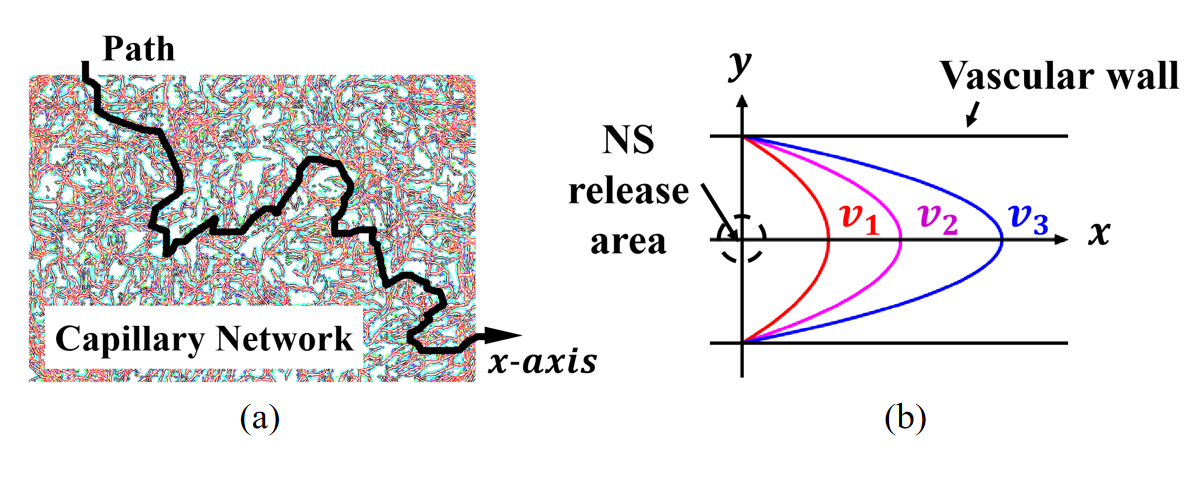
\includegraphics[width=9 cm]{fig2.png}
\caption{(a) The NS path inside the capillary network, and (b) the laminar blood flow velocity ($v_{3}>v_{2}>v_{1}$) along $x$-axis.}
\label{fig2}
\end{figure}



Given that the radius of human vessel is far less than the length of the NS trajectory, we constitute a principal $x$-axis along the tortuous trajectory of NS in the capillary network as shown in Fig. 2(a). The NS released site is the start point of the $x$-axis and the $y$-axis denotes the width of the blood vessel. The blood flow velocity is obtained by solving the Navier-Stokes equation, which provides a fundamental description of laminar flow velocity relating the pressure drop along the vessel and viscosity:

\begin{equation}
  V_f(y) = {\frac{1}{\eta}}{\frac{\Delta P}{L}}(R^{2}-y^{2}),
\label{eq1}
\end{equation}
where $V_f(y)$ is the laminar flow velocity and $y$ is the transversal distance from the $x$-axis, $R$ is the radius of the vessel, $\Delta P$ is the pressure drop along the vessel with length $L$, and $\eta$ denotes the blood viscosity. For a Newtonian fluid, the velocity profile is a parabola with the maximum value located at the center of the vessel, as shown in Fig.~\ref{fig2}(b).


\subsection {Kinematic Model of NS}
The NS state vector $\textbf{X}(t)$ is defined as a two-dimensional value $\left[ x,v_x,y,v_y \right]^{T} $, where $x$ and $v_x$ are the position and velocity respectively. The following equation illustrates the state-space relation with the mass $m$:

\begin{equation}
\label{eq0_1}
\begin{aligned}
  \begin{bmatrix}
	\dot{x}\\
	\ddot{x}\\
	\dot{y}\\
	\ddot{y}
  \end{bmatrix} =
  \textbf{A} \begin{bmatrix} x\\ \dot{x}\\ y\\ \dot{y} \end{bmatrix} +
 \textbf{B} \begin{bmatrix} u_x \\ u_y \end {bmatrix} + \textbf{W}  \boldsymbol{ \varepsilon } (t),
\end {aligned}
\end{equation}
where
\begin{equation}
\label{eq0_2}
\begin{aligned}
	\textbf{A} =  \begin{bmatrix}
		0&1&0&0\\
		0&0&0&0\\
		0&0&0&1\\
		0&0&0&0
	  \end{bmatrix},
	\textbf{B} =  \begin{bmatrix}
		 0&0 \\
	      {\frac{1}{m}}&0 \\
		 0&0 \\
		 0&{\frac{1}{m}}
	     \end{bmatrix}.
\end {aligned}
\end{equation}
The global force $\left[ u_x,u_y \right]^{T} $ denotes the input, which includes the total affections of the blood flow and the magnetic control. The Brownian noise term $ \textbf{W} \boldsymbol{\varepsilon} (t) $ is a random perturbation produced with magnitude $\textbf{W}$. The Brownian force is modelled as a Gaussian random process, thus, it is possible to estimate the NS motion with free diffusion in discrete time. The drag force of blood flow $F_d$ is modelled by the Stokes law:


\begin{equation}
\label{eq2}
\left\{
\begin{aligned}
  \gamma=6 \pi \eta a, \\
  F_d={\gamma V_f},
\end {aligned}
\right.
\end{equation}
where the friction coefficient $\gamma$ is proportional to the blood viscosity $\eta$ as the NS radius $a$ is setting to a constant value. The combination of the drag force $F_d$ and the Brownian force $F_B$ determines the acceleration and velocity of NS, which is illustrated by the generalized Langevin equations:

\begin{equation}
\label{eq3}
 \tau_B = {\frac{m}{\gamma}} \approx 10^{-3} s,
\end{equation}
and
\begin{equation}
\label{eq4}
\left\{
\begin{aligned}
  V_x'(t) + {\frac{\gamma}{m}} V_x(t) &= 
	{\frac{\gamma V_f}{m}} + {\frac{ F_{B-x} (t) }{m}},
  \\
  V_y'(t) + {\frac{\gamma}{m}} V_y(t) &= 
	 {\frac{ F_{B-y} (t) }{m}},
\end {aligned}
\right.
\end{equation}
where $\tau_B$ is the Brownian timescale for the relaxation of the NS, $ V_x(t)$ and $ V_y(t)$ are the NS velocity components along the $x$-axis and $y$-axis respectively, while $F_{B-x}(t)$ and $F_{B-y}(t)$ are the Brownian force components respectively. In general, the Brownian force is a stochastic impact of the NS performed by the surrounding molecules. The effect of the fluctuating force is given by the first and second moments:
\begin{equation}
\label{eq5}
\langle F_{B}(t) \rangle=0  ,  \langle F_{B}(t_1) , F_{B}(t_2) \rangle = 2 \gamma K_B T \delta (t_1-t_2),
\end{equation}
where $\langle \cdot \rangle$ is the average value of stochastic variables, $K_B$ is the Boltzmanns constant and $T$ is the temperature. The delta function in time indicates that there is no correlation between two time instants $t_1$ and $t_2$. In the simulation, we use a Gaussian random variable following (7) to emulate the Brownian force acting on the NS.

\subsection { Motion-based Viscosity Sensing }

Since the kinematic process of NS in the laminar flow follows the generalized Langevin equation, the measurement of blood viscosity can be reduced to a solution of a partial differential equation by removing the Brownian effects. We obtain the following formulas to calculate the blood viscosity, referring to (1), (4) and (6):

\begin{equation}
\label{eq6}
\left\{
\begin{aligned}
  \eta=
{
\frac{3 {\frac{\Delta P}{L}} \pi a (R^{2}-y^{2}) + 2 F_{B-x} – 2 m V_x }
{12 \pi a V_x}
},
  \\
  E(\eta)=
{
\frac{3 {\frac{\Delta P}{L}} \pi a (R^{2}-E(y^{2}))  – 2 m E(V_x') }
{12 \pi a E(V_x)}
},
\end {aligned}
\right.
\end{equation}
where $E(\cdot)$ is an average operator with respect to the distribution of the variables. As mentioned above, the mean Brownian force should be zero. Furthermore, there is no correlation between Brownian effects in any distinct times. Thus, the Brownian noise can be filtered by analyzing the average trajectory of NS.

In this modelling, some NS are released individually. The blood viscosity is assumed as a time-invariant value, and the parameters apart from the position and velocity in (8) are considered as constant values. Thus, it is possible to obtain the injective relation of different viscosity at different locations. The initial blood viscosity value at the released site is setting as a unit amount.  The relative viscosity, calculated by the average trajectory of NS groups  at different times, is the ratio of the location-variant viscosity to the initial value.

 
\section {LQR Controller for Sensing Enhancement}

\subsection {Location-dependent SNR}

As mentioned above, the blood viscosity is assumed as a time-invariant value. We define blood flow effects as the signal and Brownian motion as the noise, then the locaiton-dependent SNR is represented as 

\begin{equation}
  SNR = 10 {\rm log}_{10} {\frac{\vert \gamma V_f(y) V_x \vert}{\vert F_B \cdot V_x \vert} },
\label{eq7}
\end{equation}
where $\vert \gamma V_f(y) V_x \vert$ is the power of the blood flow and $\vert F_B \cdot V_x \vert $ is the power of the Brownian motion along the $x$-axis. As shown in Fig.~\ref{fig_SNR}, the sensing performance declines as the transversal distance increases. Given that a higher SNR along the path is related to a better sensing condition, this motivates us to design the controller stated in the following subsection.

\begin{figure}
\centering
\captionsetup{singlelinecheck=off}
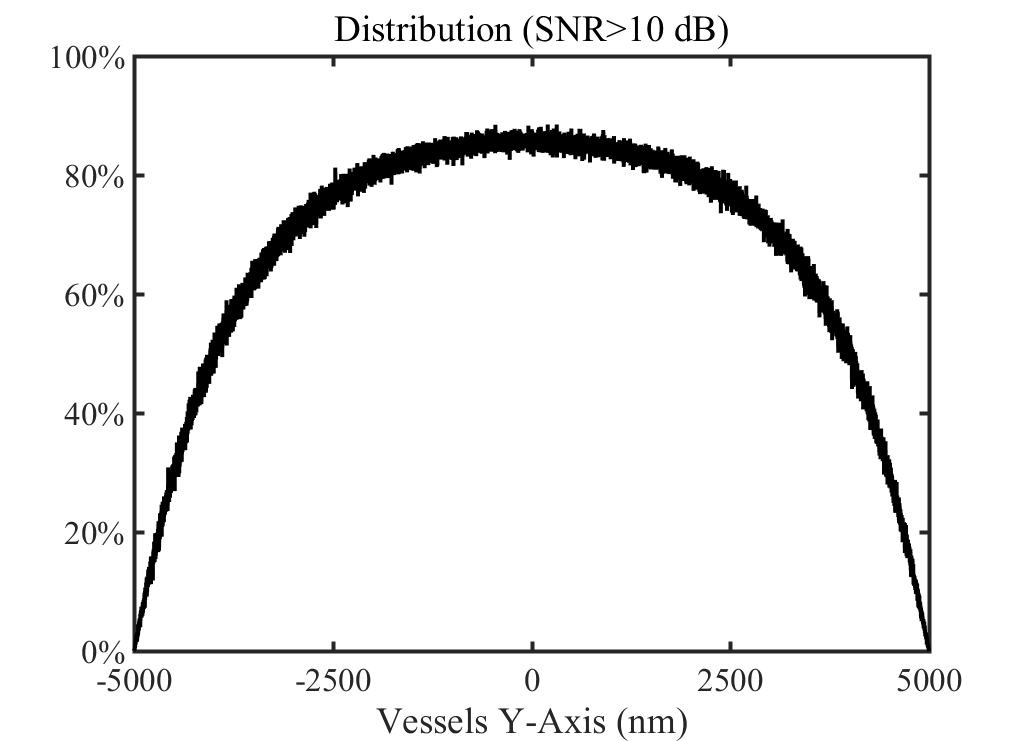
\includegraphics[width=8cm]{fig_SNR.png}
\caption{The distribution of the location-dependent SNR in the vessel.}
\label{fig_SNR}
\end{figure}

\subsection {Control Method}
We propose a real-time LQR-based automatic control method to ensure that the NS trajectory is as close to the centre of the vessel as possible. Without Brownian noise, the controllability matrix is defined as:

\begin{equation}
\label{eq8}
\begin{aligned}
	\textbf{C}&=\left[ {\textbf{B},\textbf{A}\textbf{B},\textbf{A}^{2}\textbf{B},\textbf{A}^{3} \textbf{B} } \right]\\
	& = \begin{bmatrix}
		0&0& {\frac{1}{m}}&0&0&0&0&0\\
		 {\frac{1}{m}}&0&0&0&0&0&0&0\\
		0&0&0& {\frac{1}{m}}&0&0&0&0\\
		0& {\frac{1}{m}}&0&0&0&0&0&0
	  \end{bmatrix},
\end {aligned}
\end{equation}

The full rank of (10) illustrates that a noiseless system is controllable, which is presented by the state vectors of a single NS, $\left[ x,v_x,y,v_y \right]^{T} $. Given that the Brownian noise is a time-independent Gaussian White noise, it is hard to design a complete positional controller. However, the magnitude order of magnetic force is much larger than that of Brownian motion. Thus, the impact of the Brownian force is reduced significantly by implementing a high-frequency external magnetic control. Here, LQR is introduced as an optimal controller because of its robustness and cost-effectiveness. Our target is to estimate the optimal control vector $\textbf{u}^{*}(t)$, which steers the NS along the expected trajectory. According to \cite{li2004iterative}, the performance function is defined as below:

\begin{equation}
\label{eq9}
\begin{aligned}
J(t)= &{\frac{1}{2}}\textbf{x}^{T}(t_{f})\textbf{S}\textbf{x}(t_{f}) + \\  &{\frac{1}{2}}\int_{t_{0}}^{t_{f}} \ \textbf{x}^{T}(t)\textbf{Q}\textbf{x}(t) + \textbf{u}^{T}(t)\textbf{R}\textbf{u}(t) \ dt,
\end {aligned}
\end{equation}
where $t_{0}$ is the initial time and $t_{f}$ is the end time. And the positive definite coefficient matrices $\textbf{S}$, $\textbf{Q}$ and $\textbf{R}$ are impacts on the different penalty functions as mentioned below. $L_{1}={\frac{1}{2}}\textbf{x}^{T}(t_{f})\textbf{S}\textbf{x}(t_{f}) $ represents the cost function when the controller terminates, $L_{2}=\textbf{x}^{T}(t)\textbf{Q}\textbf{x}(t) $ is the error cost function, and $L_{3}=\textbf{u}^{T}(t)\textbf{R}\textbf{u}(t) $ is the boundary condition of magnetic force. 

With parameter-tunning of the above matrixes, the optimal control vector $\textbf{u}^{*}(t)$ that minimizes $J(t)$ can be calculated by solving the Riccati equation \cite{li2004iterative}: 
\begin{equation}
\label{eq10}
\dot{\textbf{P}}(t) = -\textbf{P}(t) \textbf{A} - \textbf{A}^{T} \textbf{P}(t) - \textbf{Q} + \textbf{P}(t) \textbf{B} \textbf{R}(t)^{-1}  \textbf{B}^{T} \textbf{P}(t),
\end{equation}
and
\begin{equation}
\label{eq11}
\textbf{u}^{*}(t) = -\textbf{R}(t)^{-1} \textbf{B}^{T}\textbf{P}(t) \textbf{x}^{*}(t)  ,t\in[t_{0},t_{f}],
\end{equation}
where $\textbf{P}$(t) is a $n\times n$ positive semi-definite matrix which contributes in solving process.


\begin{table}[h]
\captionsetup{labelformat=simple, textfont=sc}
\caption{ The Simulation Parameters }
\label {table0}

\normalsize
\centering
\begin{tabular}{|c|c|}
\hline
\textbf{Parameters}                  & \textbf{Value}        \\ \hline
Blood viscosity (mPa/s)     & 1.2$\sim$2.8 \\ \hline
Vessles diameter ($\mu$m)        & 10           \\ \hline
Length of sensing path (cm) & 2            \\ \hline
$x$-axis unit length ($\mu$m)      & 1            \\ \hline
$y$-axis unit length (nm)     & 1            \\ \hline
Unit discrete time(ms)      & 0.5          \\ \hline
Frequency of controller(Hz) & 200          \\ \hline
Number of particles         & 5            \\ \hline
\end{tabular}
\end{table}


\section{Simulation Results}

In this section, the referential blood viscosity is setting as a benchmark, and the relative viscosity calculated by (8) is compared in two groups. The first group in the control of external magnetic force while the second group is not. The simulation parameters are listed in Tabel I. As shown in Fig. 4. It is obvious that the NS trajectory with a controller is close to the centre of the vessel where the location-dependent SNR is more than $10 \rm dB$. While without external control, it is a high probability that the NS would adhere to the vessel wall by the accumulated Brownian force. As shown in Fig. 5, the error of the relative viscosity is defined in $\rm dB$: 
\begin{equation}
\label{eq12}
Err(x)=10{\rm log}_{10}{\left| \frac{ Vis(x) - Vis^{*}(x) }{ Vis^{*}(x) }\right|},
\end{equation}
where $Vis^{*}(x)$ and $Vis(x)$ are the true and estimated relative viscosities, respectively. 

We can see that the error of the sensing strategy is less than $-20 \rm dB$ which means the difference between estimated relative viscosity and benchmark is less than $1\%$.  Due to NS adherence to the vessel wall without the external controller, a sharp and peak value occurs,  shown in Fig. 5(a).


\begin{figure}[htbp]
\centering

\subfigure[Without Controller]{
\begin{minipage}[]{1\linewidth}
\centering
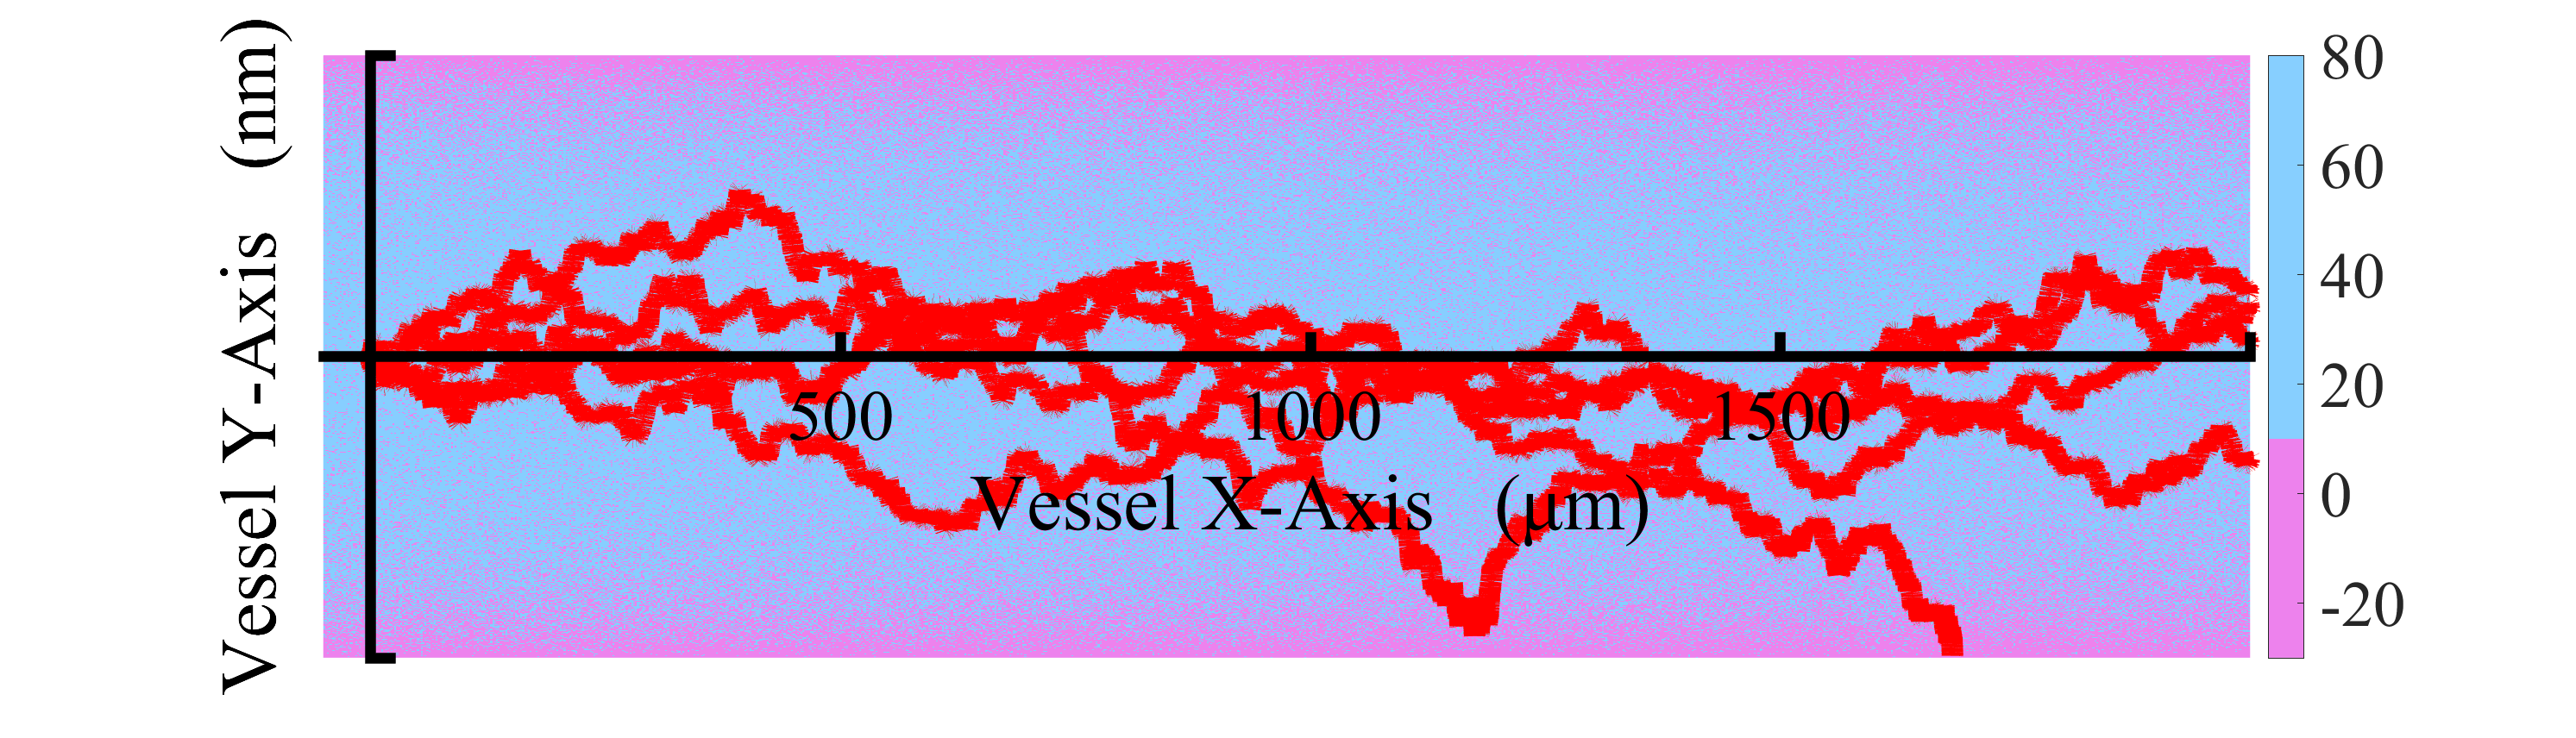
\includegraphics[width=9.5 cm]{fig3a.png}
%\caption{fig1}
\end{minipage}%
}%

\subfigure[With Controller]{
\begin{minipage}[]{1\linewidth}
\centering
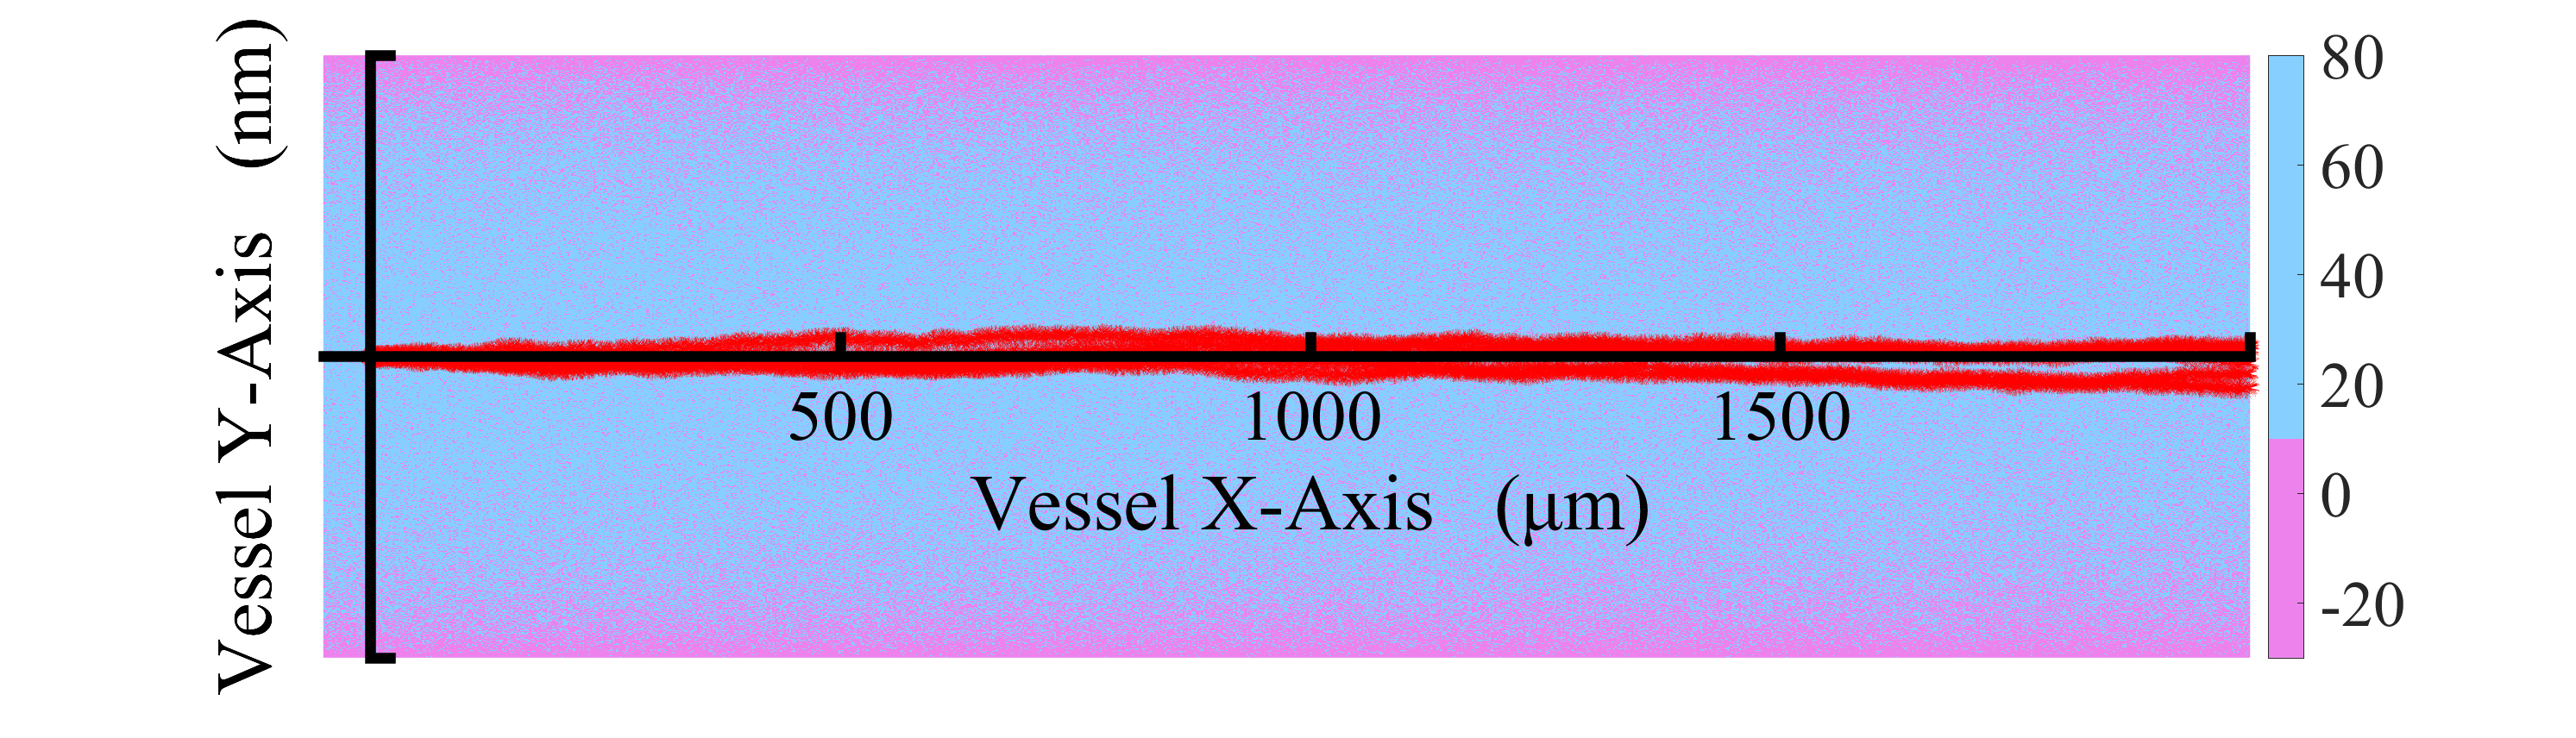
\includegraphics[width=9.5 cm]{fig3b.png}
%\caption{fig2}
\end{minipage}%
}%

\centering
\caption{The trajectorys of 5 NS: (a) without controller, and (b) with controller. And the colorbar is the location-dependent SNR (dB).}
\label {fig3}
\end{figure}

\section{Conclusion}


We have proposed a novel sensing strategy to estimate the \emph{in vivo} blood viscosity by tracking the manipulable NS; We have demonstrated through simulating that the proposed strategy can take measurements of the relative blood viscosity accurately under the external controller. Future work may include examining further the impact of non-idealities, such as the blood turbulence, imprecise tracking, and constrained steering. Finally, the proposed sensing strategy should be validated by real experiments to justify further the clinical relevance of the proposed strategy.

\begin{figure}
\centering
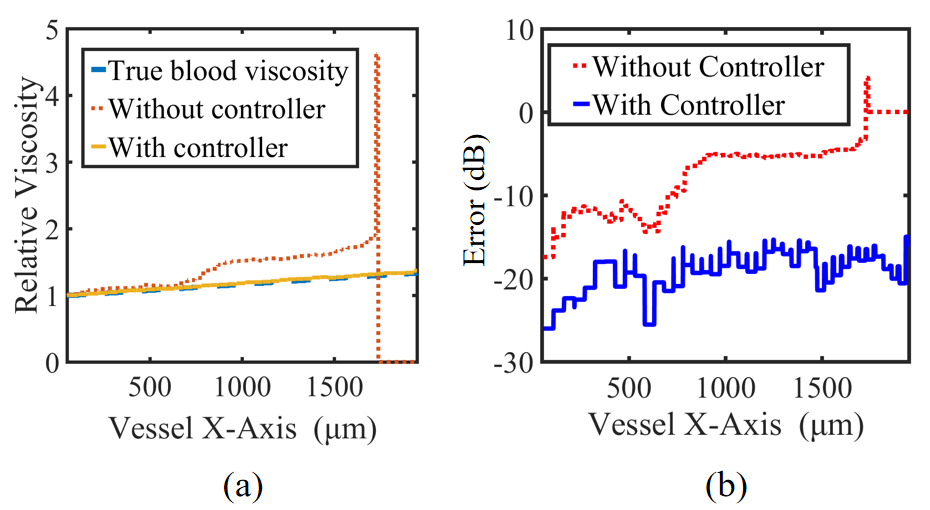
\includegraphics[width=9cm]{fig_rsterr.png}
\caption{The sensing results: (a) relative viscosity along the $x$-axis, and (b) relative error, $Err(x)$.}
\label{fig_rst}
\end{figure}


\bibliographystyle{ieeetr}
\bibliography{refe.bib}

\end{document}
